\chapter{Tactile Perception} \label{ch:1-tactile-perception}

To solve problem~\ref{prob:2} and ~\ref{prob:3}, the tactile perception solution must provide estimates of contact positions, contact normals and skew forces. \medskip

This chapter presents an analysis of the performance of different techniques to solve these problems, including a \gls{dl} model for simulating realistic tactile skew forces, and \gls{rls} for estimating contact normals. Contact normals are essential for accurately estimating the pose of an object in contact, while skew forces are critical for predicting the behavior of an object when it is grasped and manipulated by the Shadow Dexterous hand. \medskip

Firstly, the technique behind estimating the skew forces is a \gls{dl} model, which includes its architecture, is described, and the methodology used to test the network is presented. The testing methodology involves the use of various input data, and the output is analyzed for accuracy and realism. The findings are presented and discussed, including the strengths and weaknesses of the network in simulating tactile data. Finally, an assessment is made of the network's ability to produce tactile data that is realistic. \medskip

The same procedure is applied for the \gls{rls} normal estimation.\medskip

The force and normal estimates are compared to the ones provided by Gazebo's physics engine, and the known \gls{gt} from where conclusions are drawn. \medskip

The software used in this chapter is a regression neural network implemented as a Gazebo \texttt{ModelPlugin}~\cite{gazebo-model-plugin} in C++. However, the \gls{dl} model plugin used in the original publication~\cite{simulation-of-the-syntouch-biotac-sensor} has not been updated since 2018, making the code incompatible with the current version of Gazebo API. Moreover, the licensing issues with the files in the \texttt{xmlrpc++} library, which were used for base64 encoding and decoding, necessitated their removal~\cite{base64-encoding-decoding-licensing-issue}. To address these issues, each has been resolved and the plugin has been reorganized and repackaged for compatibility with the current version of Gazebo. The original version of the plugin can be found in~\cite{ruppel-philipp-biotac-gazebo-plugin}, while the fixed and updated version is available at~\cite{melbye-staven-biotac-sim-plugin}. \medskip

The availability of the updated plugin ensures that the project can continue to benefit from the capabilities of the \gls{mlp} based \gls{dl} model for simulating realistic tactile data in the current version of Gazebo.


\section{Methods}\label{sec:1-tactile-perception-method}

\subsection{Recursive Least Squares} \label{sec:1-tactile-perception-recirsive-least-squares}

To use \gls{rls} to estimate the contact normal, we require the estimated linear velocity \mvar{\hat{\vec{v}}\inR{3}}. However, since the contact points may not be consistent across the surface during motion, some points may be missing at certain time steps. To address this issue, the centroid of the contact points \mvar{\bar{\vec{c}}_t\inR{3}} is used as a representative value for each time step. Therefore, we can compute the estimated linear velocity as 
%
\begin{equation} \label{eq:v-estimate}
	\hat{\vec{v}} = \frac{\vec{\bar{c}}_{t} - \vec{\bar{c}}_{t-1}}{\Delta t},
\end{equation}

where \mvar{\bar{\vec{c}}_t\inR{3}} is the centroid of contact points in timestep \mvar{t}, \mvar{\bar{\vec{c}}_t} is the centroid for the previous timestep \mvar{t-1} and \mvar{\Delta t} is the time between samples, which in this case is \SI{0.01}{s} as the sampling frequency is \SI{100}{\hertz}. \medskip
The velocity at the fingertip in contact will then be computed as
%
\begin{equation} \label{eq:v-tip-def}
	\vec{v}_{tip} = \hat{\vec{v}} + [\bm{\omega}]_\times \rot[R]{base}{tcp} \vec{r},
\end{equation}

where \mvar{\hat{\vec{v}}} is the estimated linear velocity computed above, \mvar{[\bm{\omega}]_\times} is the skew-symmetric matrix of the angular velocity \mvar{\bm{\omega}} i.e.
%
\begin{equation} \label{eq:skew-symmetric-matrix}
	[\bm{\omega}]_\times = 
	\begin{bmatrix}
		0 & -\omega_z & \omega_y \\ \omega_z & 0 & -\omega_x \\ -\omega_y & \omega_x & 0
	\end{bmatrix} \quad , \quad \bm{\omega} = \rvec{\omega_x, \omega_y, \omega_z},
\end{equation}

\mvar{\rot[R]{base}{tcp}\inR{3\times 3}} is the rotation matrix from the hand's base to its \gls{tcp}, and \mvar{\vec{r}\inR{3}} is the position of the contact point in the base frame. \medskip

To compute the normal estimate, additionally, an initial guess is needed which is computed by
%
\begin{equation} \label{eq:def-n-init}
	\hat{\vec{n}}_{0} = \frac{\hat{\vec{v}}_{1} \times \hat{\vec{v}}_{0}}{\| \hat{\vec{v}}_{1} \times \hat{\vec{v}}_{0} \|_2},
\end{equation}
where \mvar{\hat{\vec{n}}_0\inR{3}} is the initial estimate, \mvar{\hat{\vec{v}}_{0}} and \mvar{\hat{\vec{v}}_{1}} are the linear velocity estimates for time step \num{1} and \num{0}, and \mvar{\|\cdot\|_2} is the \mvar{\ell_2}-norm. \medskip

Using the quantities above, the two main components \mvar{\mat{L}_n^1\inR{3\times 3}} and \mvar{\mat{L}_n^2\inR{3\times 3}} of the desired estimate \mvar{\hat{\vec{n}}_{new}\inR{3}} can be found. Firstly, \mvar{\mat{L}_n^1} is computed as
%
\begin{equation} \label{eq:def-L-n-1}
	\mat{L}_n^1 = \mat{L}_n^1 - \beta \Delta t \mat{L}_n^1 + \frac{\Delta t K_L}{1+\|\vec{v}_{tip}\|_2^2} \vec{v}_{tip} \vec{v}_{tip}^\T,
\end{equation}
with \mvar{\beta\inR{}} being a decay factor, \mvar{K_L\inR{}} is a gain and \mvar{\|\cdot\|_2^2} is the squared \mvar{\ell_2}-norm. \medskip

The second component \mvar{\mat{L}_n^2} is computed by
%
\begin{equation} \label{eq:def-L-2}
	\mat{L}_n^2 = \mat{L}_n^2 - \beta \Delta t \mat{L}_n^2 + \frac{\Delta t K_L}{1+
	\|\vec{\nabla}\|_2^2} \vec{\nabla} \vec{\nabla}^\T,
\end{equation}
where \mvar{\vec{\nabla}\inR{3}} is the cross product between the contact force \mvar{\vec{f}_c} and th velocity of the tip \mvar{\vec{v}_{tip}} i.e.
%
\begin{equation} \label{eq:def-nabla-rls}
	\vec{\nabla} = \vec{f}_c \times \vec{v}_{tip}.
\end{equation}
Using these components a \gls{pd} controller is used to compute the change in normal \mvar{\dot{\vec{n}}\inR{3}} as 
%
\begin{equation} \label{eq:def-n-dot}
	\dot{\vec{n}} = -\left( \gamma_1 \mat{L}_n^1 + \gamma_2 \mat{L}_n^2 \right)\vec{n},
\end{equation}
where \mvar{\gamma_1} is the proportional gain, \mvar{\gamma_2} is the derivative gain and \mvar{\vec{n}} is the current estimate. By computing the cross product between \mvar{\vec{n}} and \mvar{\dot{\vec{n}}}, the angular velocity \mvar{\vec{\omega}} is computed
%
\begin{equation} \label{eq:omega-from-n-and-n-dot}
	\vec{\omega} = \vec{n} \times \dot{\vec{n}}.
\end{equation}
Finally, the new normal estimate \mvar{\vec{n}_{new}\inR{3}} can be computed as
%
\begin{equation}
	\vec{n}_{new} = e^{ \left[ \frac{\Delta t }{2} [\vec{\omega}]_\times \right]} \vec{n},
\end{equation}
where \mvar{e^{ \left[ \frac{\Delta t }{2} [\vec{\omega}]_\times \right]}\inR{3\times 3}} is the exponential map of the skew-symmetric matrix represents the rotation due to the angular velocity over the time step.

\subsection{Network Architecture}\label{sec:1-tactile-perception-method-network-architecture}
% wrap
In~\cite{simulation-of-the-syntouch-biotac-sensor} two different architectures were built, where architecture B is chosen due to its better greater accuracy and lower execution time. The network architecture B can be seen in~\figref{fig:dl-model-tactile-perception}. As inputs, the network takes one contact position \mvar{\vec{c} = \rvec{c_x, c_y,c_z}} along with three force vector samples \mvar{\vec{f}_{1}=\rvec{f_{1,x},f_{1,y},f_{1,z}}}, \mvar{\vec{f}_{2}=\rvec{f_{2,x},f_{2,y},f_{2,z}}} and \mvar{\vec{f}_{3}=\rvec{f_{3,x},f_{3,y},f_{3,z}}}, and a temperature input \mvar{T\inR{}}, which makes the input \mvar{\rvec{\vec{c},\vec{f}_1,\vec{f}_2,\vec{f}_3,T}\inR{13}}. The outputs of the network are the data format produced by the physical sensor i.e. an output vector of \mvar{\rvec{pdc, pac, tdc, tac, e_1, \dots, e_{19}}\inR{23}}, where \mvar{pdc} is the pressure DC signal, \mvar{pac} is the pressure AC signal, \mvar{tdc} is the temperature DC signal, \mvar{tac} is the temperature AC signal and \mvar{e_1} to \mvar{e_{19}} are the electrode activations.

The network architecture consists of four \gls{mlp}s, one for interpreting the position input, one for interpreting the force inputs, one for interpreting the temperature input, and one for combining the interpretations of force and position inputs. \gls{mlp} \num{1}, responsible for interpreting the position data, consists of four hidden layers, three of which contain \num{512} neurons and uses \gls{relu} as the activation function, while the fourth and last uses a linear activation function with \num{64} neurons. The activation functions can be seen marked red if they use \gls{relu}, green if they use a linear activation function and blue if they use a sigmoid activation function. \medskip

\gls{mlp} \num{2} interprets the force inputs but rather than using \num{512}, uses \num{256} for its hidden layers, while still having the linear activation function and the \num{64} neurons in its fourth layer. This \gls{mlp} further differs as the \num{256} neuron layers apply \mvar{\ell_1} bias regularization. \gls{mlp} \num{3} produces a temperature correction vector using two hidden layers, one with \num{256} neurons and a sigmoid activation function and one with \num{23} neurons and a linear activation function. The last \gls{mlp}, \gls{mlp} \num{4} takes in the element-wise product of \gls{mlp} \num{1} and \num{2}, parses the product through two \num{256} neuron layers with \gls{relu} and one \num{23} neuron layer with a linear activation function.\medskip

The products of \gls{mlp} \num{3} and \num{4} are summed and parsed as the model's output.


% which is incorporated to achieve the final output vector. The temperature correction vector, comprising a densely connected layer of 256 neurons with sigmoid activation for smooth temperature regression and a reduction layer with linear activation, set to output size.

% The position and force inputs are handled by two distinct \gls{mlp}s, each comprising three densely connected layers with \gls{relu} activation. To enable accurate differentiation between various areas on the sensor surface, the position column employs \num{512} neurons per layer, whereas the force column employs \num{256} neurons per layer with \mvar{\ell_1} bias regularization. 

% Both columns conclude with a smaller output layer of 64 neurons with linear activation. The outputs of the position and force columns are multiplied together, and the product is processed through two densely connected layers with ReLU activation, each containing 256 neurons. The result is then reduced to output size by a smaller densely connected layer with linear activation. Finally, a temperature correction vector is incorporated to achieve the final output vector. The temperature correction vector is created by a third column, comprising a densely connected layer of 256 neurons with sigmoid activation for smooth temperature regression and a reduction layer with linear activation, set to output size.

% Initially, a densely connected sequential model (referred to as Network A) was developed, with five hidden layers of sizes 1024, 4096, 512, 512, and 512 and a ReLU activation function. Various experiments with different layer sizes, counts, and activation functions were conducted before settling on this configuration.

\begin{figure}[h]
		\begin{center}
			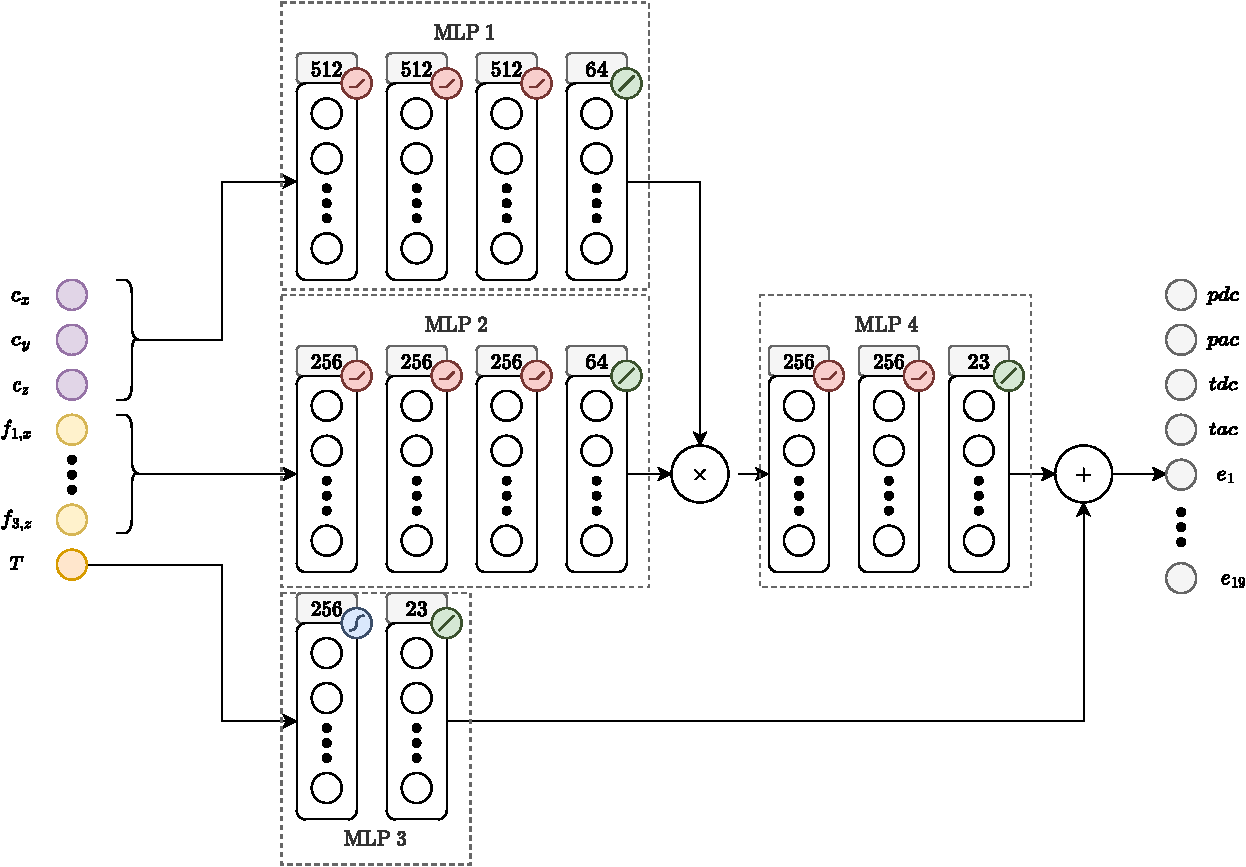
\includegraphics[width=\textwidth]{chapters/1-tactile-perception/fig/drawio/dl-model-tactile-perception-grouping-crop.pdf}
		\end{center}
		\caption{\gls{dl} model B from~\cite{simulation-of-the-syntouch-biotac-sensor}, which also has provided inspiration for this illustration.}
		\label{fig:dl-model-tactile-perception}
\end{figure}


\subsection{Network Training Procedure}\label{sec:1-tactile-perception-method-network-training-procedure}

The model presented in~\secref{sec:1-tactile-perception-method-network-architecture} was trained using a custom dataset collected by the authors. The dataset \mvar{D} contains \mvar{N_{dp} = \num{300 000}} tactile sensor readings, consisting of the complete BioTac sensor data as well as the applied reference forces. This can be seen below

\begin{equation} \label{eq:dl-data-matrix}
	D =
	\left[\begin{array}{@{}c|cccccccccccccc@{}}
		0       & pcd & pac & tdc & tac & e_{1} & \cdots & e_{19} & f_{1,x} & \cdots & f_{3,z} & c_x & c_y & c_z \\
		1       & pcd & pac & tdc & tac & e_{1} & \cdots & e_{19} & f_{1,x} & \cdots & f_{3,z} & c_x & c_y & c_z \\
		\vdots  &  &  &  &  &  &  & \vdots &  &  &  &  &  &  \\
		N_{dp}  & pcd & pac & tdc & tac & e_{1} & \cdots & e_{19} & f_{1,x} & \cdots & f_{3,z} & c_x & c_y & c_z
		\end{array}\right] \inR{N_{dp} \times 35}
\end{equation}

All inputs are normalized to have zero mean and unit variance, based on the distribution of the captured data. The three force vectors are sampled at intervals of \SI{100}{\milli\second} to prevent overfitting and avoid unrealistic reactions to high-frequency inputs that the physics simulator cannot replicate. The BioTac sensor electrode values exhibit a non-linear dependence on device temperature and attempts to correct this before inputting the data resulted in poor performance. Instead, the network was trained to compensate for this dependency by itself. During simulation, a constant temperature was assumed, which is typically the average temperature of the training set. The network generates simulated electrode and pressure signals as outputs but does not currently simulate temperature outputs. \medskip

The forces were collected using a calibrated six-axis force-torque sensor~\cite{ati:-6-axis-force-and-torque-sensor-nano17-series} with a nominal force resolution better than \SI{0.01}{\newton}. 

The contact position is reconstructed optically using a calibrated HD webcam and two AprilTag markers~\cite{apriltag:-a-robust-and-flexible-visual-fiducial-system}, one mounted on the BioTac and one attached to the probe object. The setup for this can be seen in \figref{fig:biotac-sim-experimental-setup}. Once the contact positions were collected, optimization-based calibrations were made to gain more accurate position estimates. \medskip

The data set has been made publicly available and can be found in~\cite{biotac-dataset}.

\begin{figure}[h]
	\begin{center}
		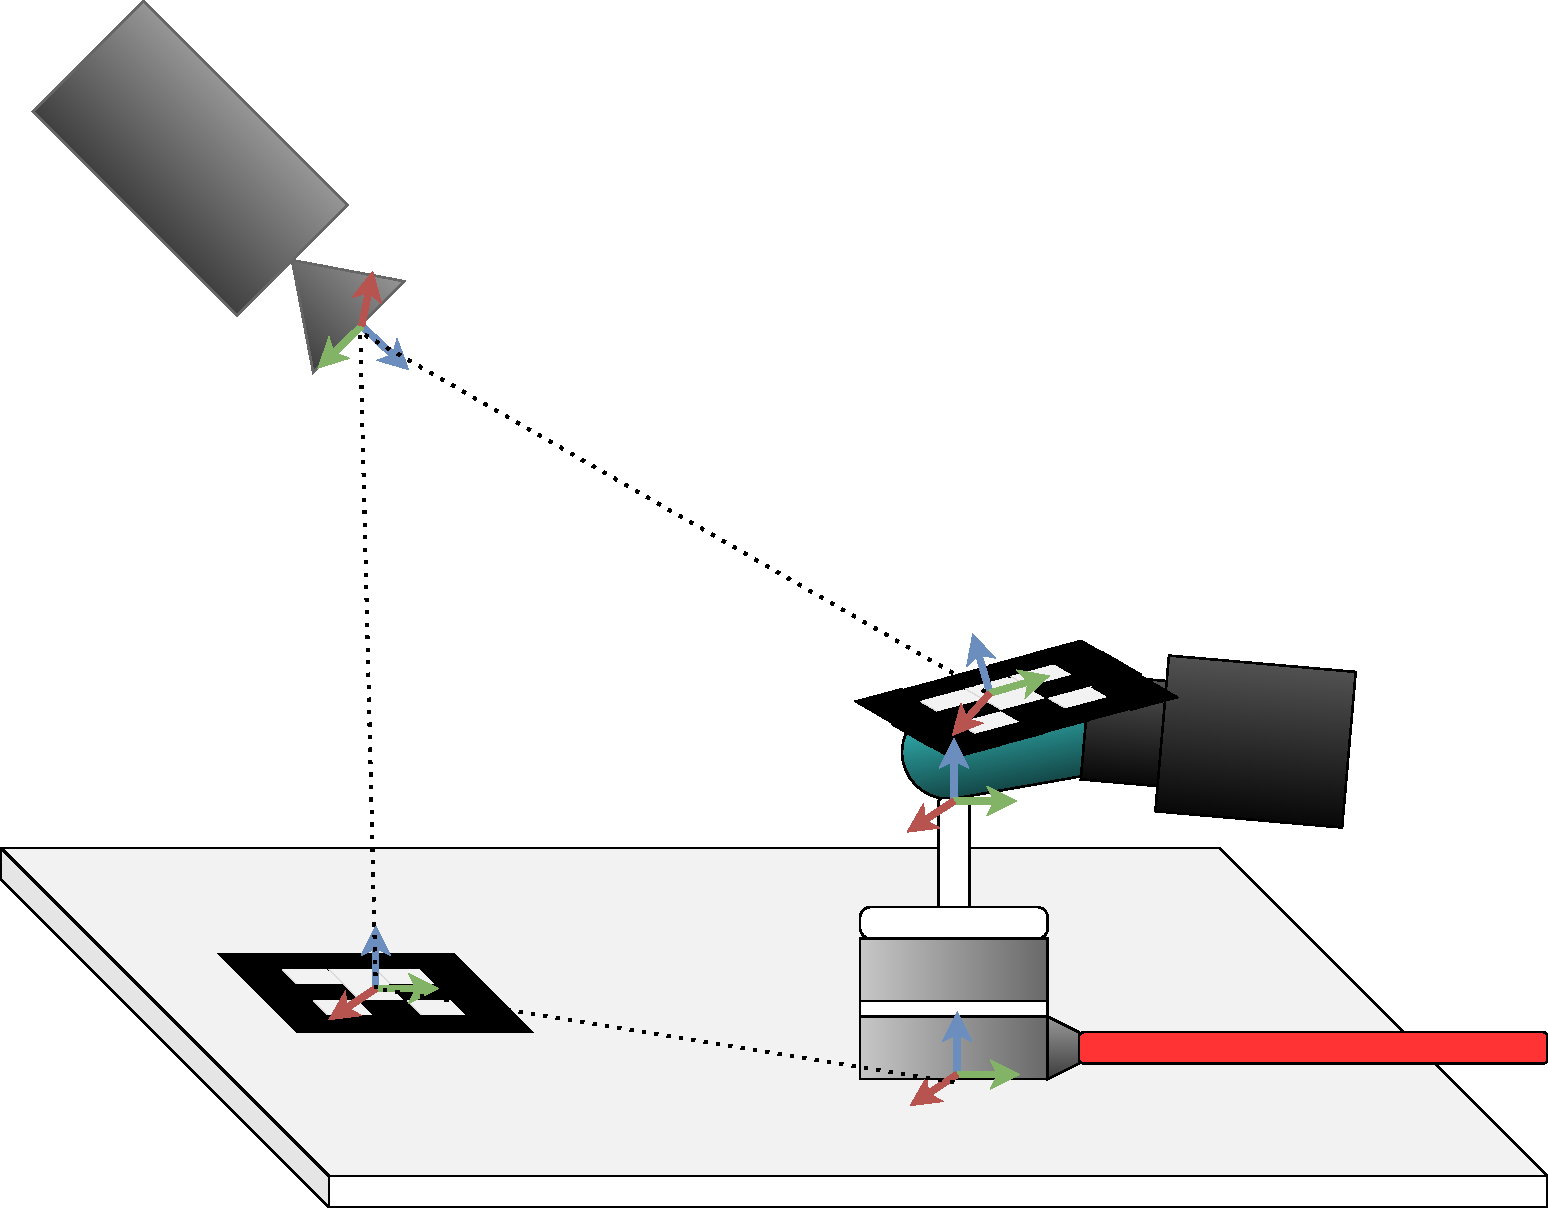
\includegraphics[width=0.7\textwidth]{chapters/1-tactile-perception/fig/drawio/biotac-sim-experimental-setup.pdf}
	\end{center}
	\caption{Experimental setup for gathering data to train \gls{dl} model B, as inspired by~\cite{simulation-of-the-syntouch-biotac-sensor}.}
	\label{fig:biotac-sim-experimental-setup}
\end{figure}

\section{Experimental Setup}\label{sec:1-tactile-perception-experimental-setup}


\subsection{Contact Normal Estimation}\label{sec:1-tactile-perception-experimental-setup-contact-normal-estimation}

To test the \gls{rls} method's ability to estimate contact normals the index finger makes contact with a flat surface as shown in~\figref{fig:normal-flat-contact-3d}, through flexion and ulnar deviation a contact path is created as shown in~\figref{fig:2d-projected-contact-path-across-flat-surface}. The motion is done throughout \SI{14}{\second}, and due to a significant presence of noise, the contact position data is filtered using a rolling low pass filter with window size \num{100}. The experiment was conducted with the finger on the surface facing \mvar{-\vec{y}}, meaning the \gls{gt} normal is \mvar{\vec{n}_{gt}=\rvec{0,-1,0}}.

\begin{figure}[h]
	\centering
	\begin{subfigure}[b]{0.48\textwidth}
		\centering
		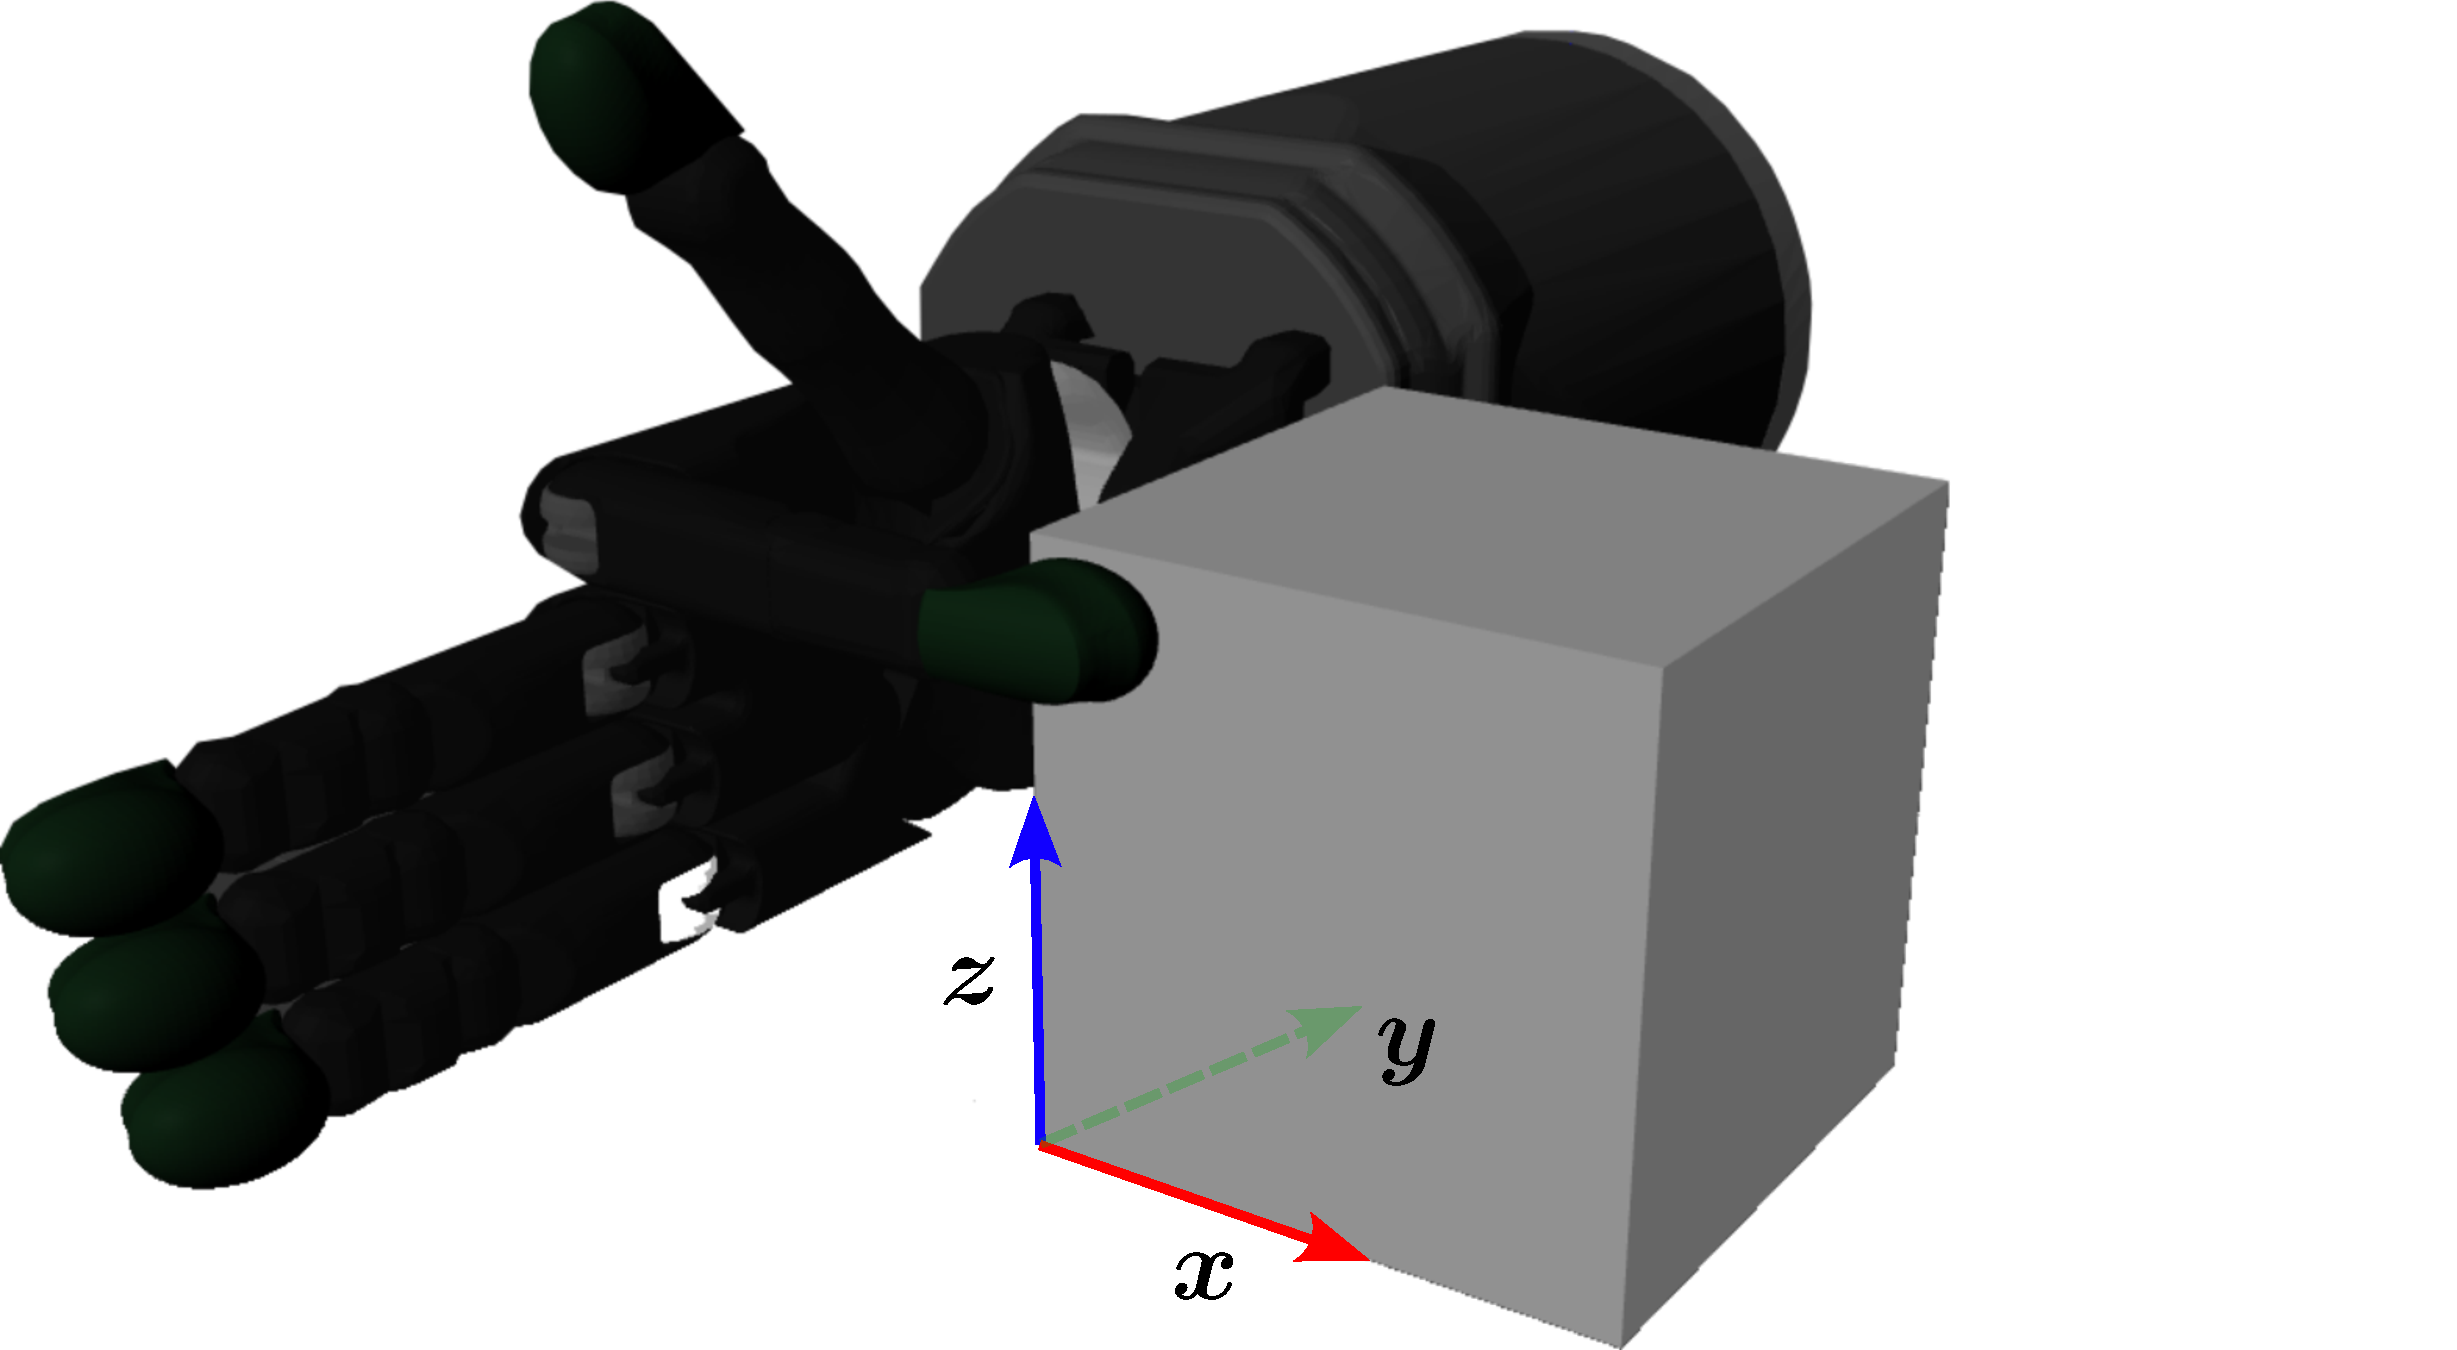
\includegraphics[width=\textwidth]{chapters/1-tactile-perception/fig/inkscape/flat-contact-coor.pdf}
		\caption{Map showing a 2D projection of the electrodes' positions and numbers.}
		\label{fig:normal-flat-contact-3d}
	\end{subfigure}
	\hfill
	\begin{subfigure}[b]{0.48\textwidth}
		\centering
		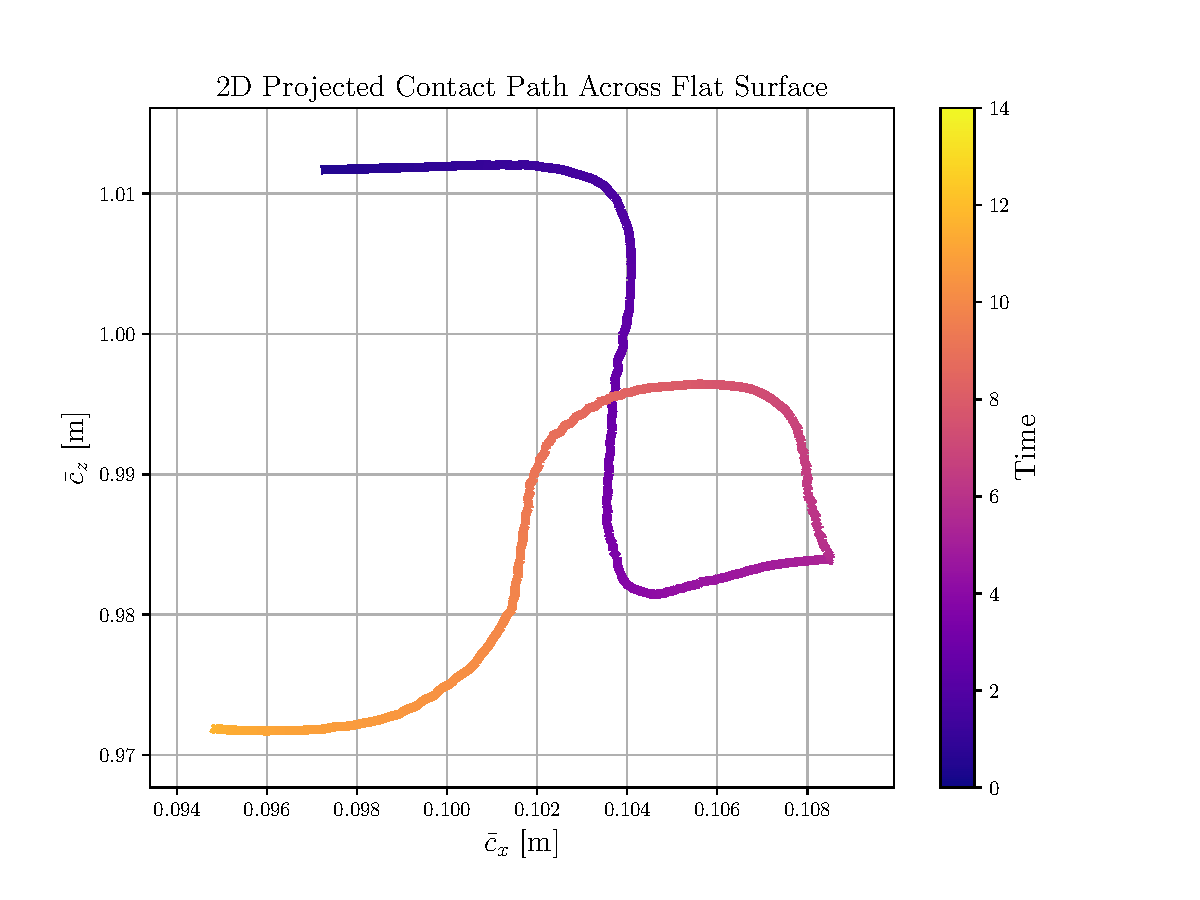
\includegraphics[width=\textwidth]{chapters/1-tactile-perception/fig/matplotlib/2d-projected-contact-path-across-flat-surface.pdf}
		\caption{3D plot of electrode activations when the Shadow Dexterous hand's index finger makes contact with a flat surface.}
		\label{fig:2d-projected-contact-path-across-flat-surface}
	\end{subfigure}
		\caption{3D plot of electrode activations and 2D electrode map with labels.}
		\label{fig:experimental-setup-for-normal-estimation}
\end{figure}


\subsection{Skew Force Estimation}\label{sec:1-tactile-perception-experimental-setup-skew-force-estimation}

To test the performance of the \gls{dl} model, four objects surfaces were used with known normals. These can be seen in~\figref{fig:experimental-setup-tactile-perception} as a flat surface, an edge, a smooth surface and a corner.

\begin{figure}[h]
	\centering
	\begin{subfigure}[b]{0.24\textwidth}
		\centering
		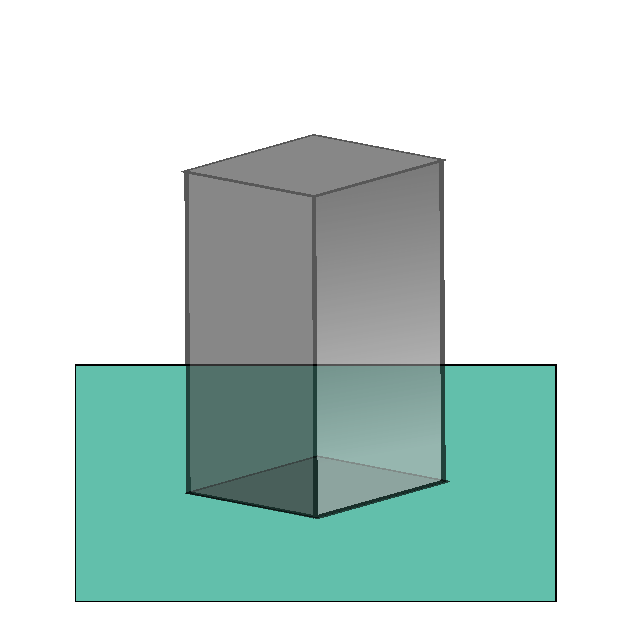
\includegraphics[width=\textwidth]{chapters/1-tactile-perception/fig/inkscape/flat-contact-3d.pdf}
		\caption{Finger in contact with a flat surface.}
		\label{fig:flat-contact}
	\end{subfigure}
	\hfill
	\begin{subfigure}[b]{0.24\textwidth}
		\centering
		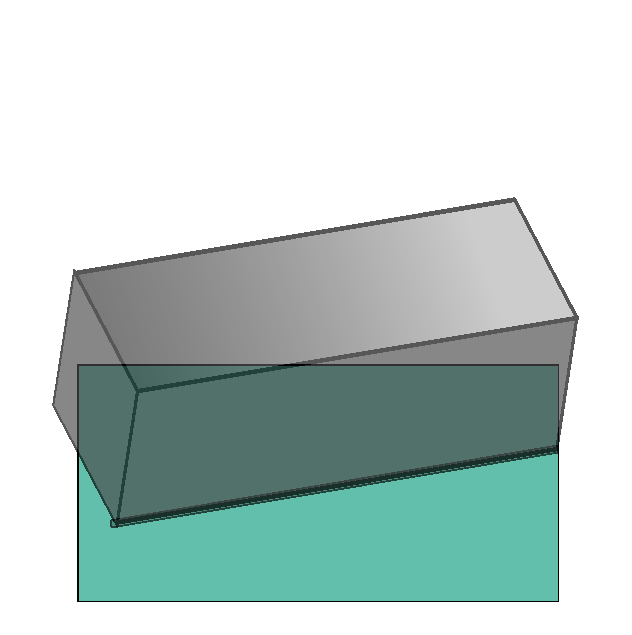
\includegraphics[width=\textwidth]{chapters/1-tactile-perception/fig/inkscape/edge-contact-3d.pdf}
		\caption{Finger in contact with an edge. \newline}
		\label{fig:edge-contact}
	\end{subfigure}
	\hfill
	\begin{subfigure}[b]{0.24\textwidth}
		\centering
		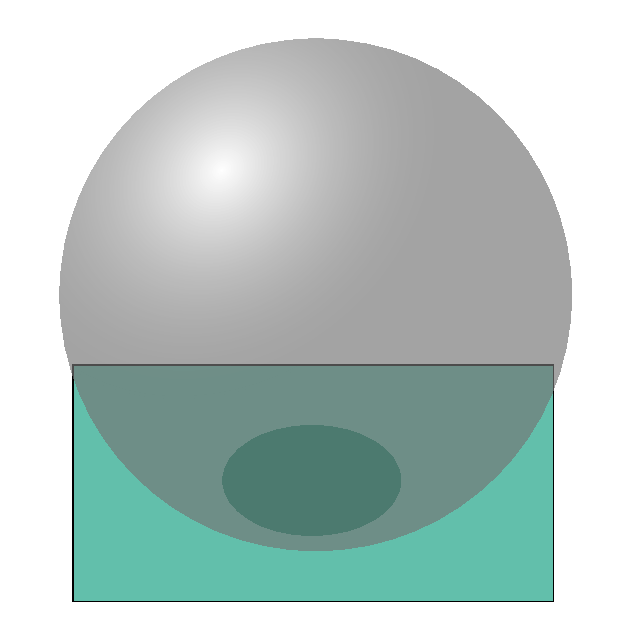
\includegraphics[width=\textwidth]{chapters/1-tactile-perception/fig/inkscape/smooth-contact-3d.pdf}
		\caption{Finger in contact with a smooth surface.}
		\label{fig:smooth-contact}
	\end{subfigure}
	\hfill
	\begin{subfigure}[b]{0.24\textwidth}
		\centering
		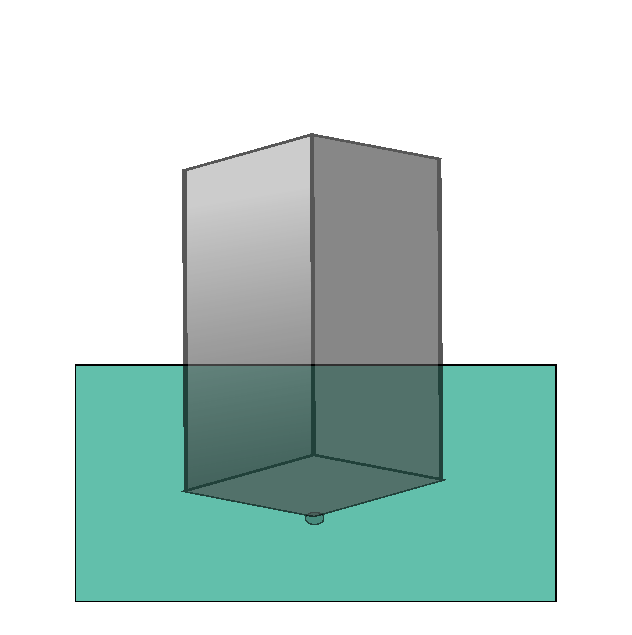
\includegraphics[width=\textwidth]{chapters/1-tactile-perception/fig/inkscape/corner-contact-3d.pdf}
		\caption{Finger in contact with a corner.\newline}
		\label{fig:corner-contact}
	\end{subfigure}
		\caption{The four surfaces used to test the performance of the \gls{dl} model's ability to represent surfaces.}
		\label{fig:experimental-setup-tactile-perception}
\end{figure}

Within the simulation, the index finger is set to make contact with each surface, as shown in~\figref{fig:experimental-setup-tactile-perception-experimental}.
\begin{figure}[h]
	\centering
	\begin{subfigure}[b]{0.24\textwidth}
		\centering
		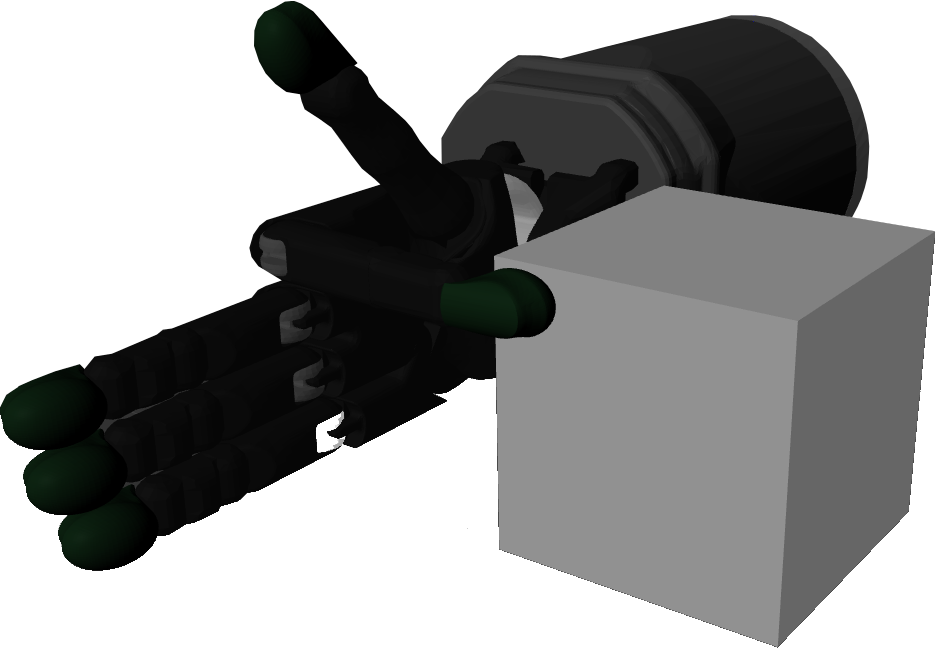
\includegraphics[width=\textwidth]{chapters/1-tactile-perception/fig/screen-shots/flat-contact-crop.png}
		\caption{Simulated index finger in contact with a flat surface.}
		\label{fig:flat-contact-experimental}
	\end{subfigure}
	\hfill
	\begin{subfigure}[b]{0.24\textwidth}
		\centering
		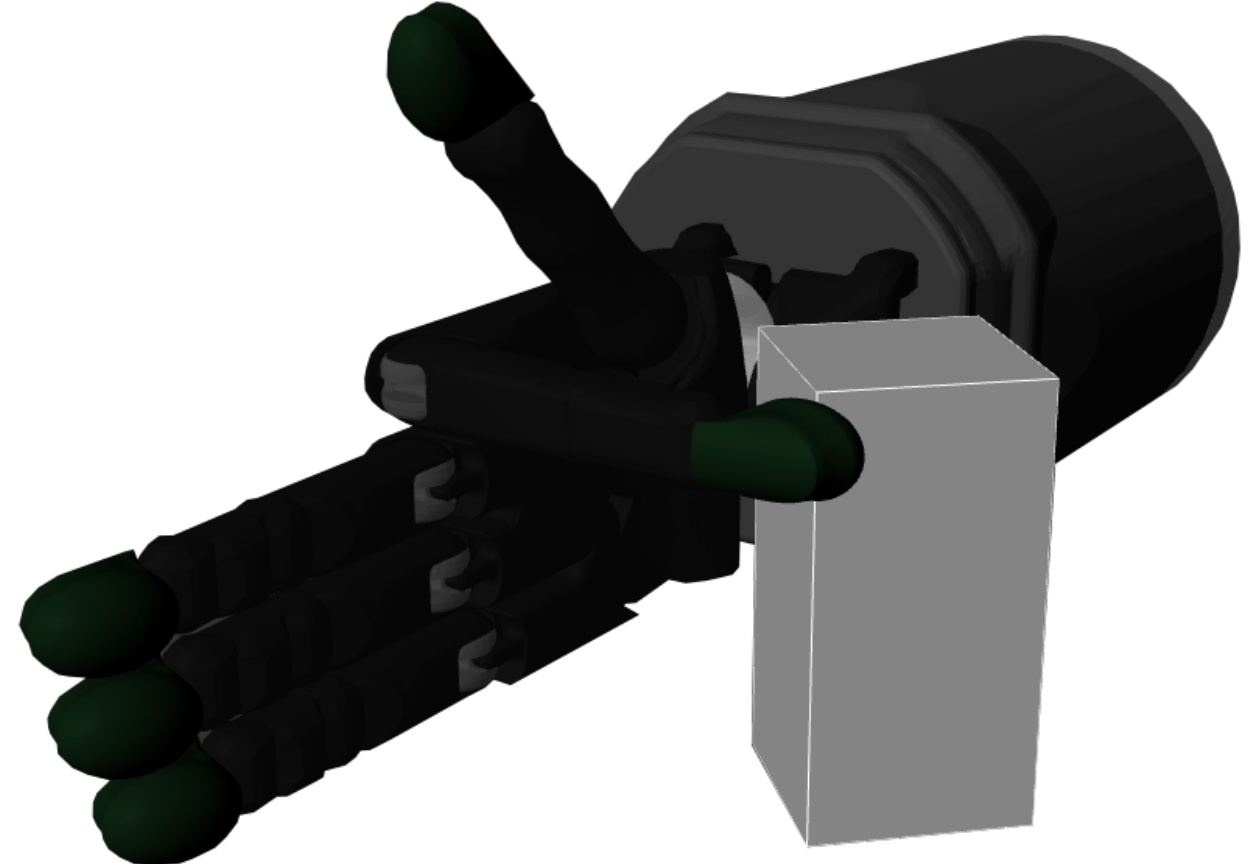
\includegraphics[width=\textwidth]{chapters/1-tactile-perception/fig/screen-shots/edge-contact.png}
		\caption{Simulated index finger in contact with an edge.}
		\label{fig:edge-contact-experimental}
	\end{subfigure}
	\hfill
	\begin{subfigure}[b]{0.24\textwidth}
		\centering
		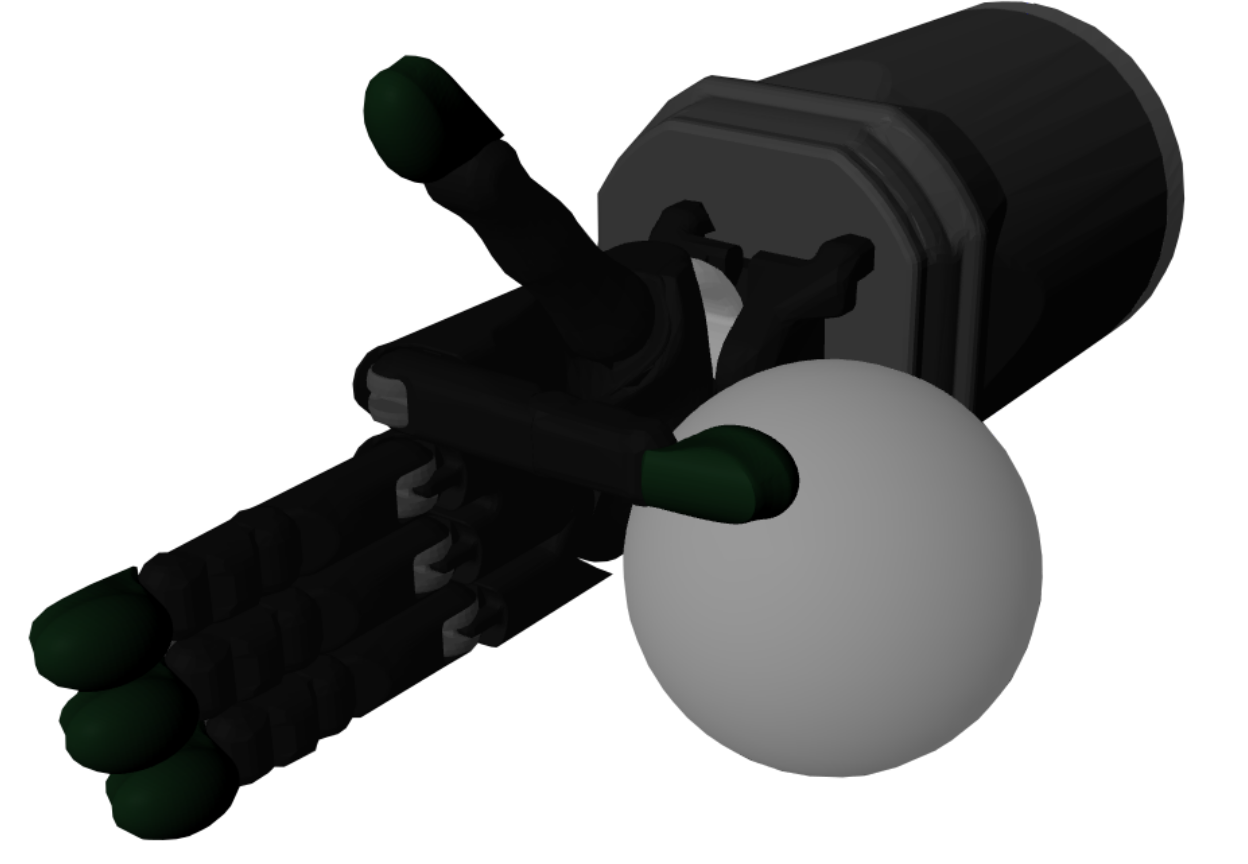
\includegraphics[width=\textwidth]{chapters/1-tactile-perception/fig/screen-shots/smooth-contact.png}
		\caption{simulated index finger in contact with a smooth surface.}
		\label{fig:smooth-contact-experimental}
	\end{subfigure}
	\hfill
	\begin{subfigure}[b]{0.24\textwidth}
		\centering
		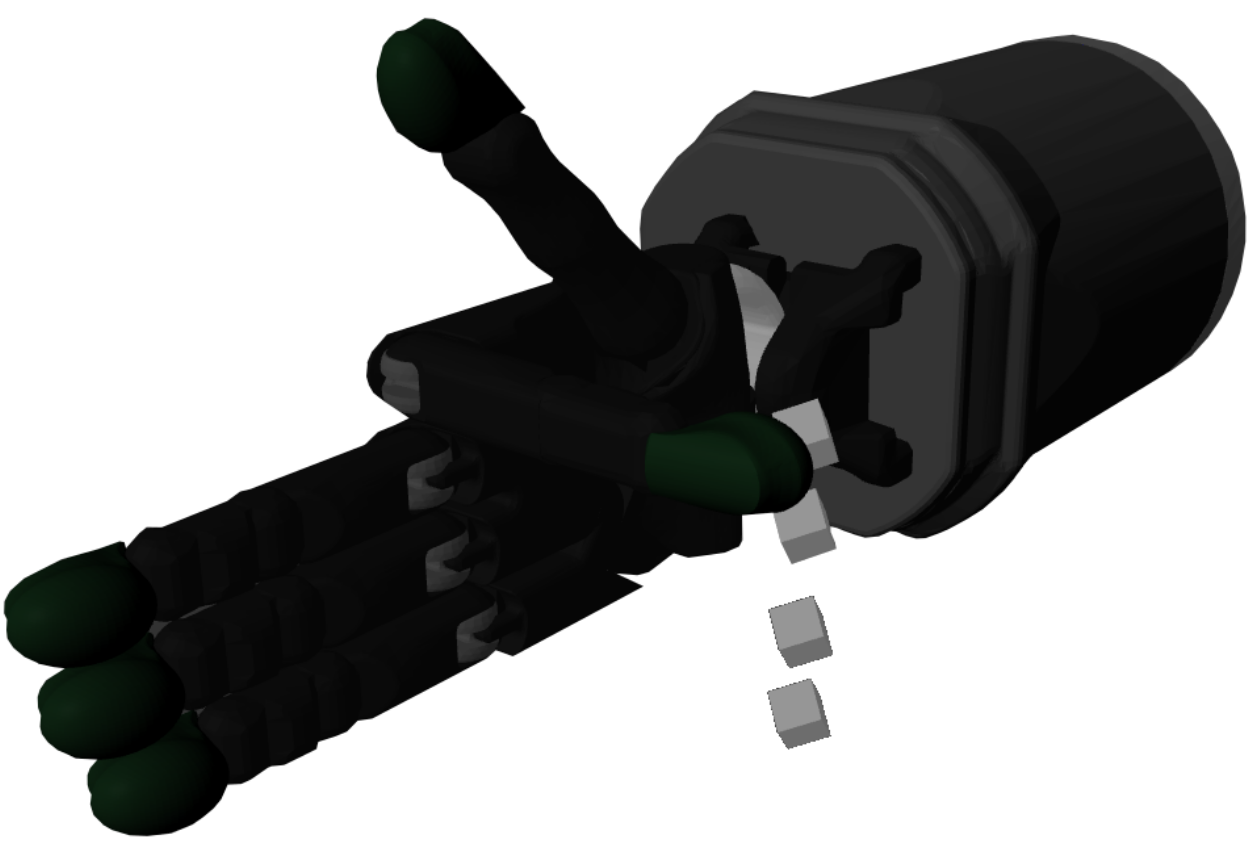
\includegraphics[width=\textwidth]{chapters/1-tactile-perception/fig/screen-shots/corner-contact.png}
		\caption{Simulated index finger in contact with a corner}
		\label{fig:corner-contact-experimental}
	\end{subfigure}
		\caption{The simulated Shadow Dexterous hand in contact with the four surfaces used to test the performance of the \gls{dl} model's ability to represent surfaces. In each case, the contact is made by the index finger.}
		\label{fig:experimental-setup-tactile-perception-experimental}
\end{figure}

When contact is made the inputs and outputs of the \gls{dl} model are recorded over \SI{30}{\second}, which with a sampling frequency of \SI{100}{\hertz} results in \num{3000} samples. As inputs are collected, the contact positions and forces are given by Gazebo in \robframe{W}, which then is transformed into the contact frame \robframe{C} using the grasping matrix \mat{G}, to ensure consistency. Due to contact data in Gazebo being prone to noise, an exponential decay filter is additionally applied.

% ground truth vectors presented on figures and how errors were computed

% holding bunny, and logging forces. Forces compared to the theoretical ideal.

% as a solution, one can train an object detection NN for converting tactile data into contact points and normals.

\section{Results}\label{sec:1-tactile-perception-results}

After executing the \gls{dl} model on all cases, the resulting simulated electrode activations were discovered to be infinite. Consequently, efforts were undertaken to address this issue. It was determined that the model does not include layer-wise normalization to establish limits on feature responses. The addition of this normalization procedure resulted in the network outputting values within the expected range.~\figref{fig:simulated-electrode-distribution} shows a 3D plot of the electrode activations, while~\figref{fig:electrode-map} shows a 2D projection of the finger tip with its labeled electrodes.

\begin{figure}[h]
	\centering
	\begin{subfigure}[b]{0.48\textwidth}
		\centering
		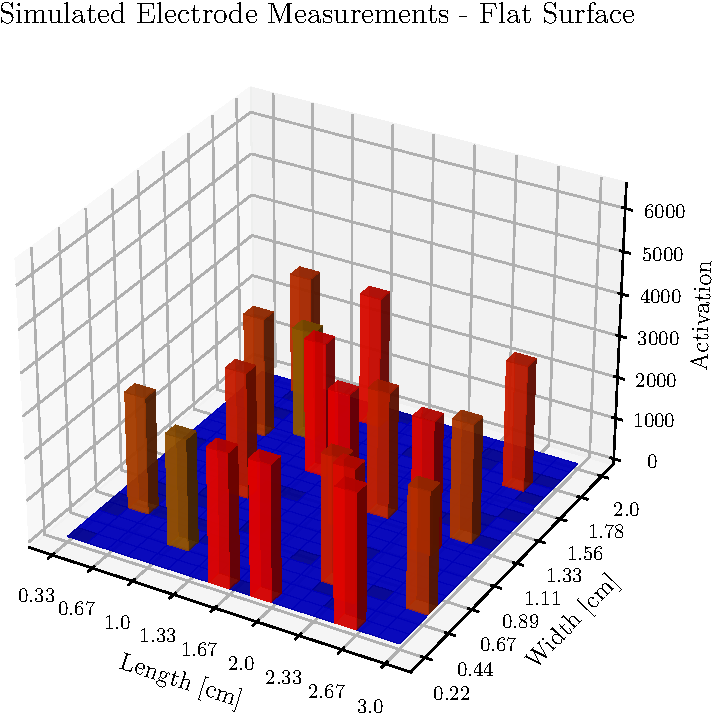
\includegraphics[width=\textwidth]{chapters/1-tactile-perception/fig/matplotlib/pressure-distribution.pdf}
		\caption{3D plot of electrode activations when the Shadow Dexterous hand's index finger makes contact with a flat surface.}
		\label{fig:simulated-electrode-distribution}
	\end{subfigure}
	\hfill
	\begin{subfigure}[b]{0.48\textwidth}
		\centering
		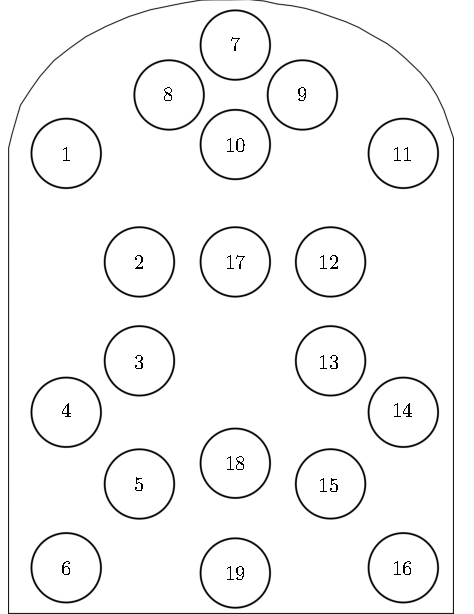
\includegraphics[height=\textwidth]{chapters/1-tactile-perception/fig/drawio/electrode-map.pdf}
		\caption{Map showing a 2D projection of the electrodes' positions and numbers.}
		\label{fig:electrode-map}
	\end{subfigure}
		\caption{3D plot of electrode activations and 2D electrode map with labels.}
		\label{fig:flat-contact-experimental-and-electrode-map}
\end{figure}

\subsection{Contact Normals} \label{sec:1-tactile-perception-results-contact-normals}

Upon estimating the linear velocities~\figref{fig:linear-velocity-finger-in-contact-with-flat-surface} was produced, which shows the three velocity components. Due to a great presence of noise, a rolling low pass filter was applied with a window size of \num{100}. As one would expect the \mvar{v_y} is of negligible magnitude, as shown here. \medskip

\begin{figure}[!h]
	\begin{center}
		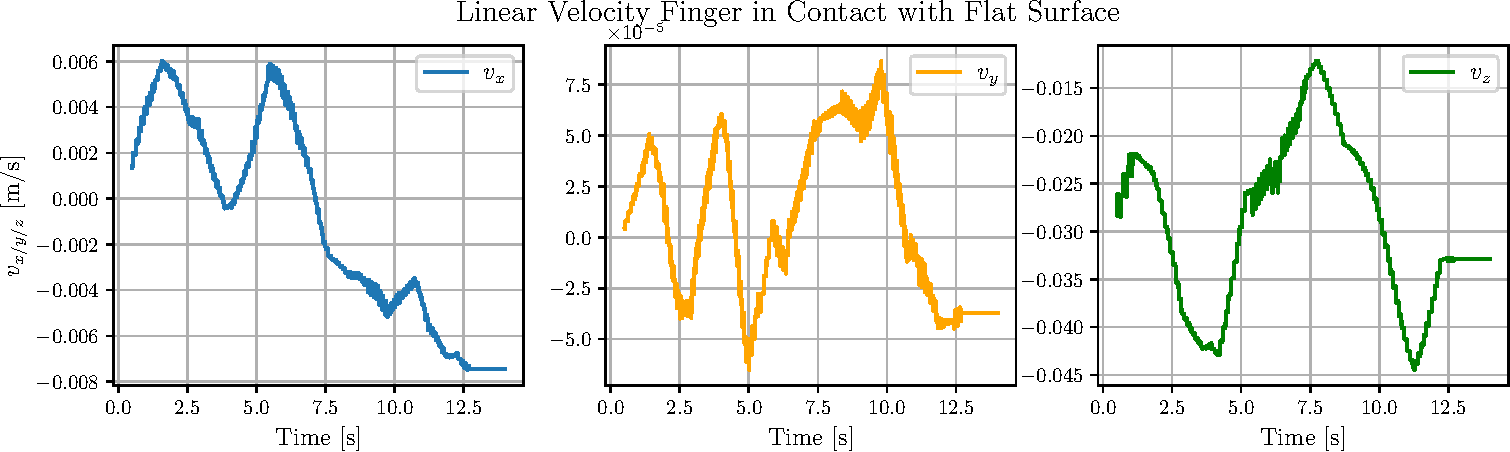
\includegraphics[width=\textwidth]{chapters/1-tactile-perception/fig/matplotlib/linear-velocity-finger-in-contact-with-flat-surface.pdf}
	\end{center}
	\caption{The simulated tactile electrode activations.}
	\label{fig:linear-velocity-finger-in-contact-with-flat-surface}
\end{figure}

Based on these the contact normals are estimated using \gls{rls}, which results in~\figref{fig:contact-normal-estimates}, which show great consistency and accuracy.

\begin{figure}[!h]
	\begin{center}
		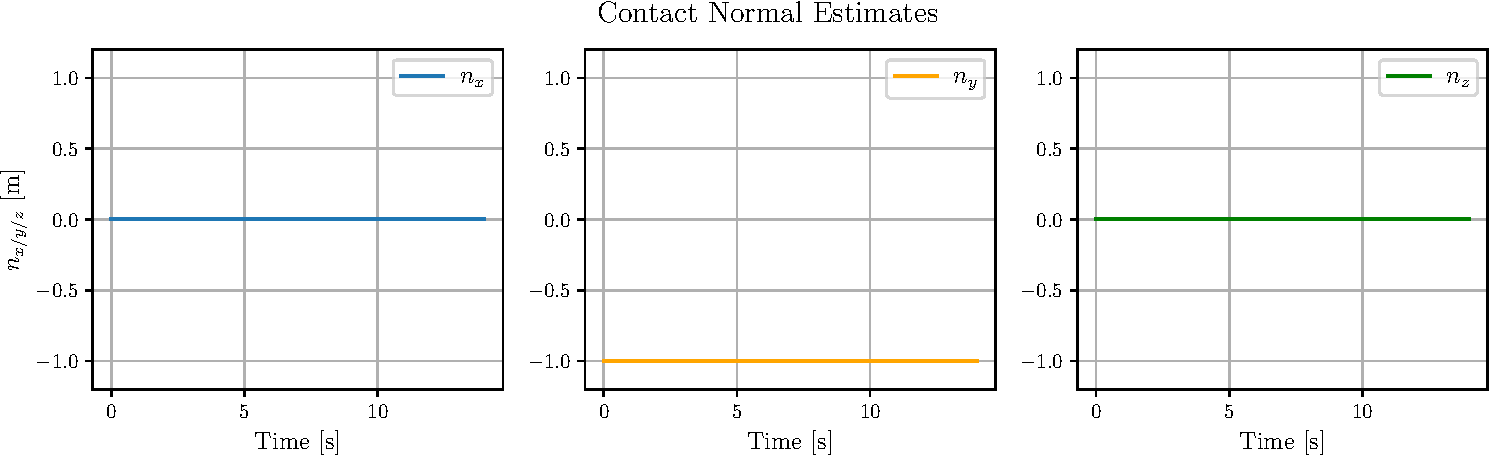
\includegraphics[width=\textwidth]{chapters/1-tactile-perception/fig/matplotlib/contact-normal-estimates.pdf}
	\end{center}
	\caption{The simulated tactile electrode activations.}
	\label{fig:contact-normal-estimates}
\end{figure}

\subsection{Skew Forces} \label{sec:1-tactile-perception-results-skew-forces}

\figref{fig:flat-contact-graph} illustrates the inputs and outputs of the \gls{dl} model when the Shadow Dexterous hand's index finger makes contact with a flat surface. As seen here, the output of the model is independent of the input. To verify this behavior, data from the data set on which the model has been trained is applied and a similar result is found as seen in~\figref{fig:train-contact-graph}. \medskip

Due to this independence of input, the electrodes, and by extension the \gls{dl} model is not judged to be able to accurately simulate skew forces for a BioTac sensor in contact. The contact data from the remaining experiments can be found in~\appref{app:tactile-perception-simulated-electrode-activations}, which show a similar pattern.

\begin{figure}[!h]
	\begin{center}
		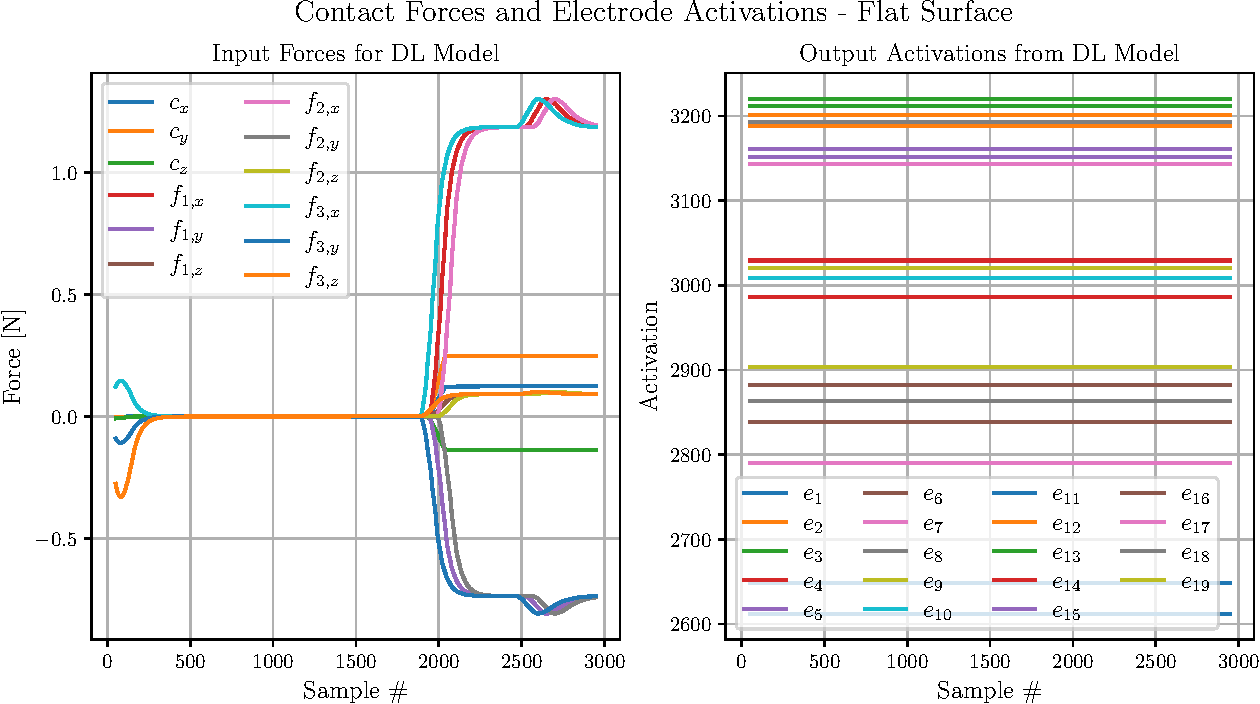
\includegraphics[width=\textwidth]{chapters/1-tactile-perception/fig/matplotlib/flat-contact-graph.pdf}
	\end{center}
	\caption{The simulated tactile electrode activations.}
	\label{fig:flat-contact-graph}
\end{figure}
\begin{figure}[!h]
	\begin{center}
		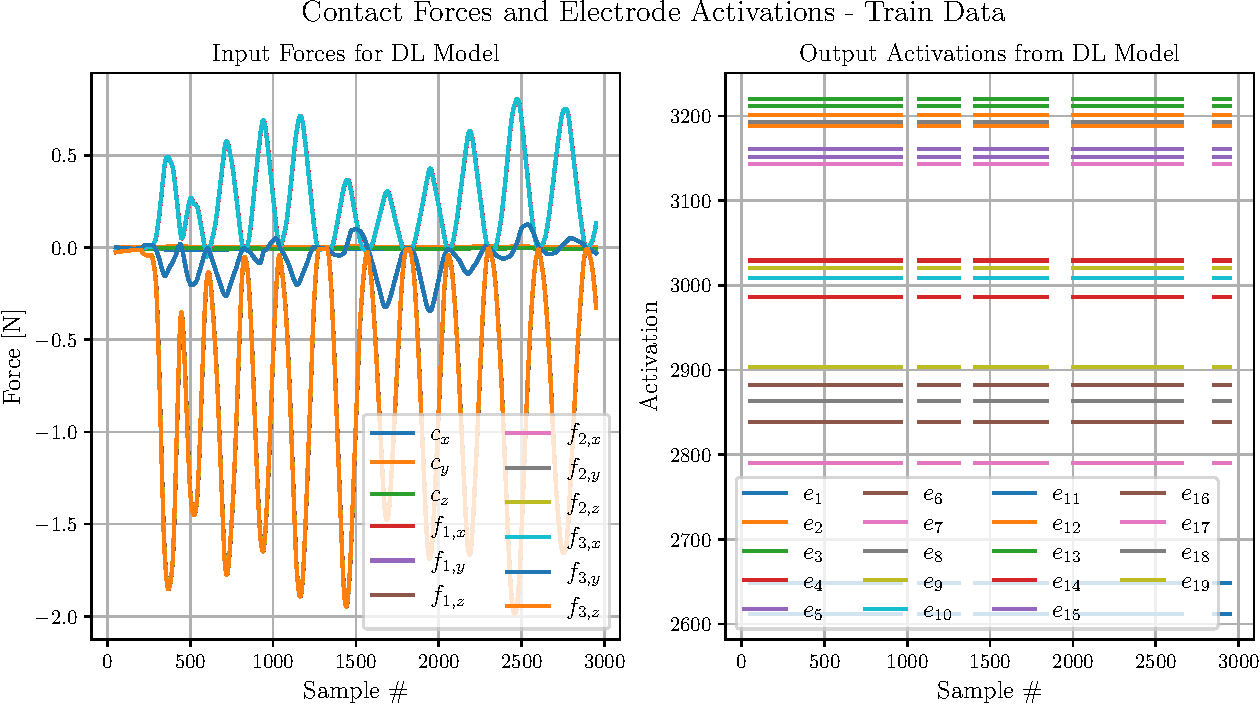
\includegraphics[width=\textwidth]{chapters/1-tactile-perception/fig/matplotlib/train-contact-graph.pdf}
	\end{center}
	\caption{The simulated tactile electrode activations.}
	\label{fig:train-contact-graph}
\end{figure}

\subsection{Gazebo Physics Engine Comparison}\label{sec:1-tactile-perception-results-gazebo-comparison}




Engine 

\begin{figure}[h]
	\centering
	\begin{subfigure}[b]{0.48\textwidth}
		\centering
		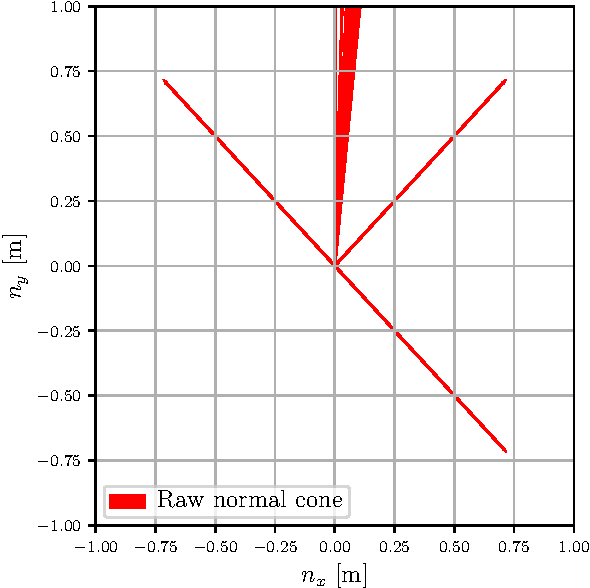
\includegraphics[width=\textwidth]{chapters/1-tactile-perception/fig/matplotlib/xy-projected-raw-normal-cones.pdf}
		\caption{3D plot of electrode activations when the Shadow Dexterous hand's index finger makes contact with a flat surface.}
		\label{fig:simulated-electrode-distribution3}
	\end{subfigure}
	\hfill
	\begin{subfigure}[b]{0.48\textwidth}
		\centering
		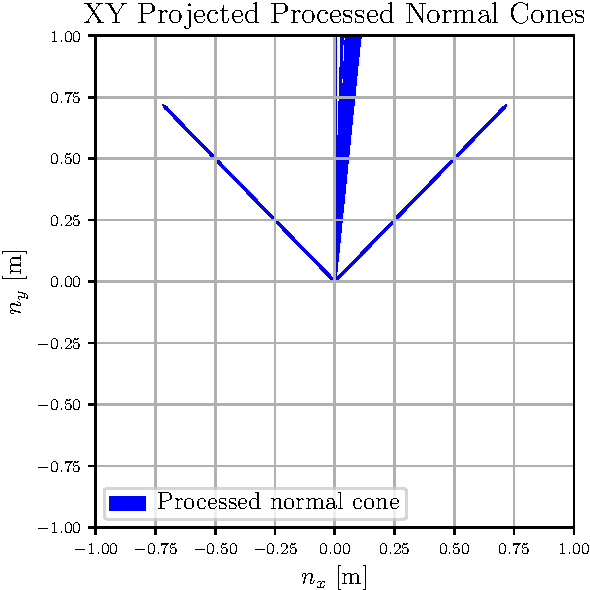
\includegraphics[width=\textwidth]{chapters/1-tactile-perception/fig/matplotlib/xy-projected-processed-normal-cones.pdf}
		\caption{Map showing a 2D projection of the electrodes' positions and numbers.}
		\label{fig:electrode-map3}
	\end{subfigure}
		\caption{3D plot of electrode activations and 2D electrode map with labels.}
		\label{fig:flat-contact-experimental-and-electrode-map3}
\end{figure}


\begin{figure}[h]
	\centering
	\begin{subfigure}[b]{0.48\textwidth}
		\centering
		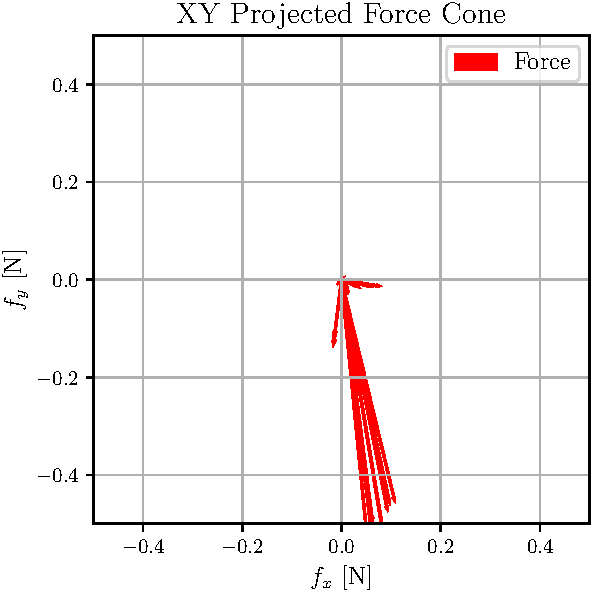
\includegraphics[width=\textwidth]{chapters/1-tactile-perception/fig/matplotlib/xy-projected-force-cones.pdf}
		\caption{3D plot of electrode activations when the Shadow Dexterous hand's index finger makes contact with a flat surface.}
		\label{fig:simulated-electrode-distribution2}
	\end{subfigure}
	\hfill
	\begin{subfigure}[b]{0.48\textwidth}
		\centering
		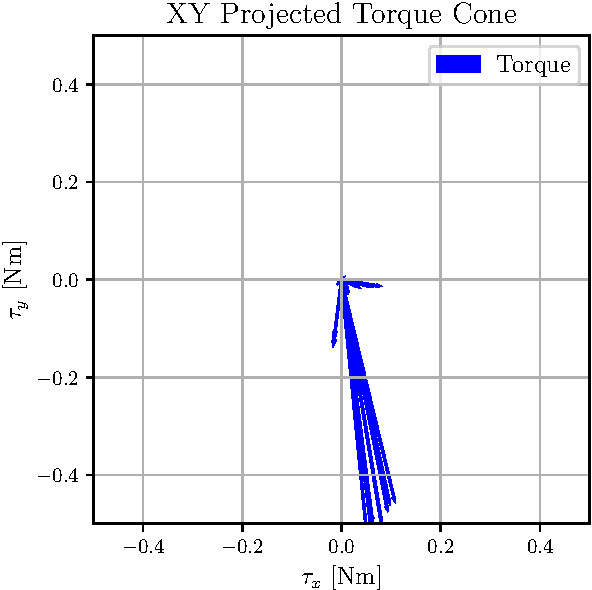
\includegraphics[width=\textwidth]{chapters/1-tactile-perception/fig/matplotlib/xy-projected-torque-cones.pdf}
		\caption{Map showing a 2D projection of the electrodes' positions and numbers.}
		\label{fig:electrode-map2}
	\end{subfigure}
		\caption{3D plot of electrode activations and 2D electrode map with labels.}
		\label{fig:flat-contact-experimental-and-electrode-map2}
\end{figure}



\section{Discussion \& Conclusion}\label{sec:1-tactile-perception-discussion-and-conclusion}

It seems to represent the real phenomenons realistically 


% \section{Related Work} \label{sec:1-tactile-perception-related-work}

% Here we cite the related work by \texttt{\textbackslash cite\{source-label\}} like this \cite{recent-progress-in-technologies-for-tactile-sensors}